\documentclass{article}
\usepackage{pgf-umlcd}
\begin{document}
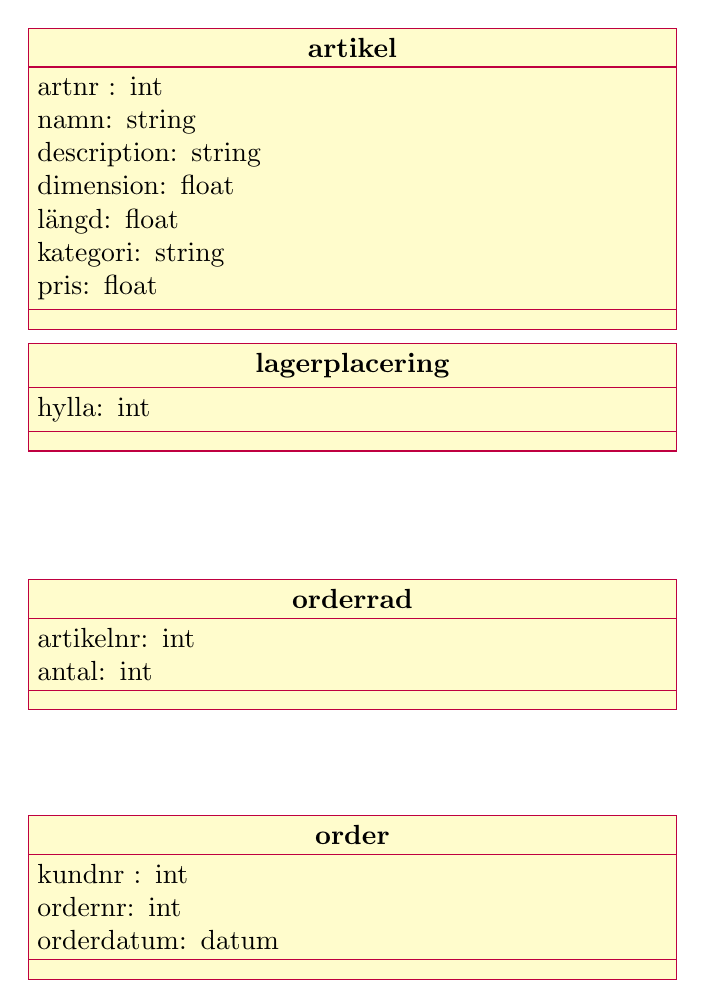
\begin{tikzpicture}

  \begin{class}[text width=8cm]{order}{0,0}
    \attribute{kundnr : int}
    \attribute{ordernr: int}
    \attribute{orderdatum: datum}
  \end{class}

  \begin{class}[text width=8cm]{order}{0,0}
    \attribute{kundnr : int}
    \attribute{ordernr: int}
    \attribute{orderdatum: datum}
  \end{class}

  \begin{class}[text width=8cm]{orderrad}{0,3}
    \attribute{artikelnr: int}
    \attribute{antal: int}
  \end{class}

  \begin{class}[text width=8cm]{lagerplacering}{0,6}
    \attribute{hylla: int}
  \end{class}

  \begin{class}[text width=8cm]{artikel}{0,10}
    \attribute{artnr : int}
    \attribute{namn: string}
    \attribute{description: string}
    \attribute{dimension: float}
    \attribute{längd: float}
    \attribute{kategori: string}
    \attribute{pris: float}
  \end{class}

\end{tikzpicture}
